\chapter{Method} \label{CH4}
Run simulations of plates with defects using cheap FSI by multiplying the lagrangian pressure with cosine of angle. Train a ANN and see if it can replicate this cheap FSI, (it should pretty much 100\%). Integrate the neural net with abaqus.

Simulate the plate using fully coupled FSI in Europlexus. Train an AI on this. Evaluate. Investigate if the material properties can be accounted for in the neural net.

\begin{figure}
    \centering
    \begin{subfigure}[b]{0.6\textwidth}
        \centering
        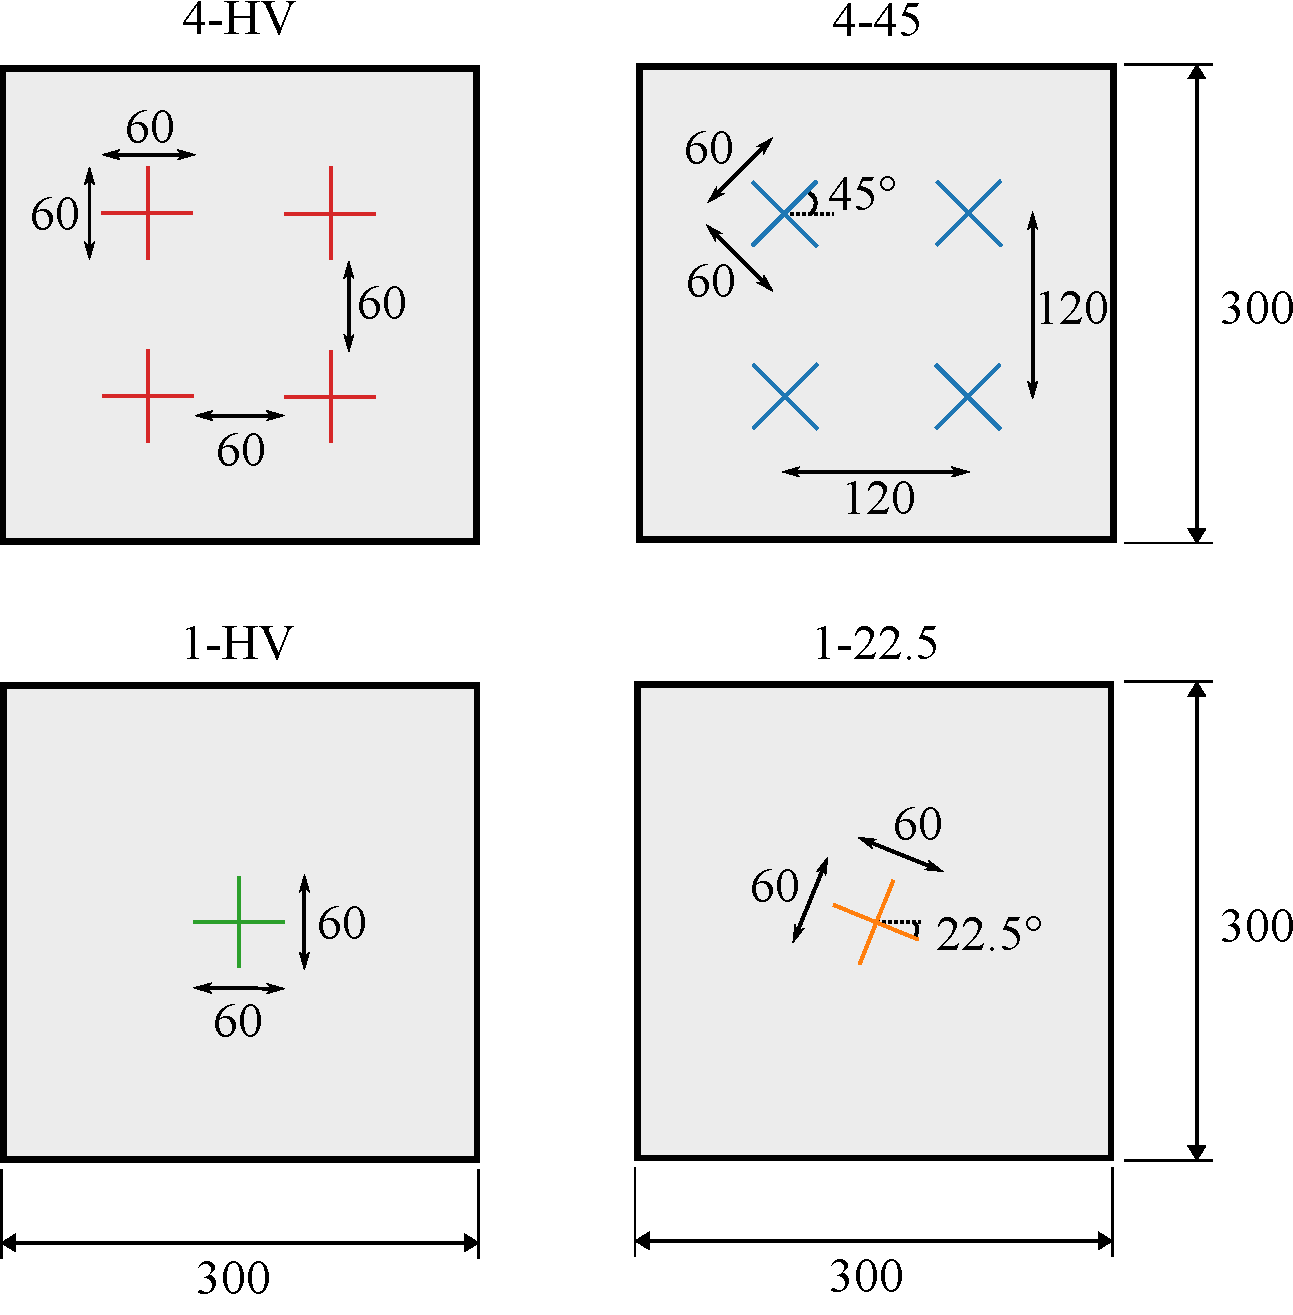
\includegraphics[width=\textwidth]{plates}
        \caption{}
        \label{fig:plates}
    \end{subfigure}
    \begin{subfigure}[b]{0.39\textwidth}
        \centering
        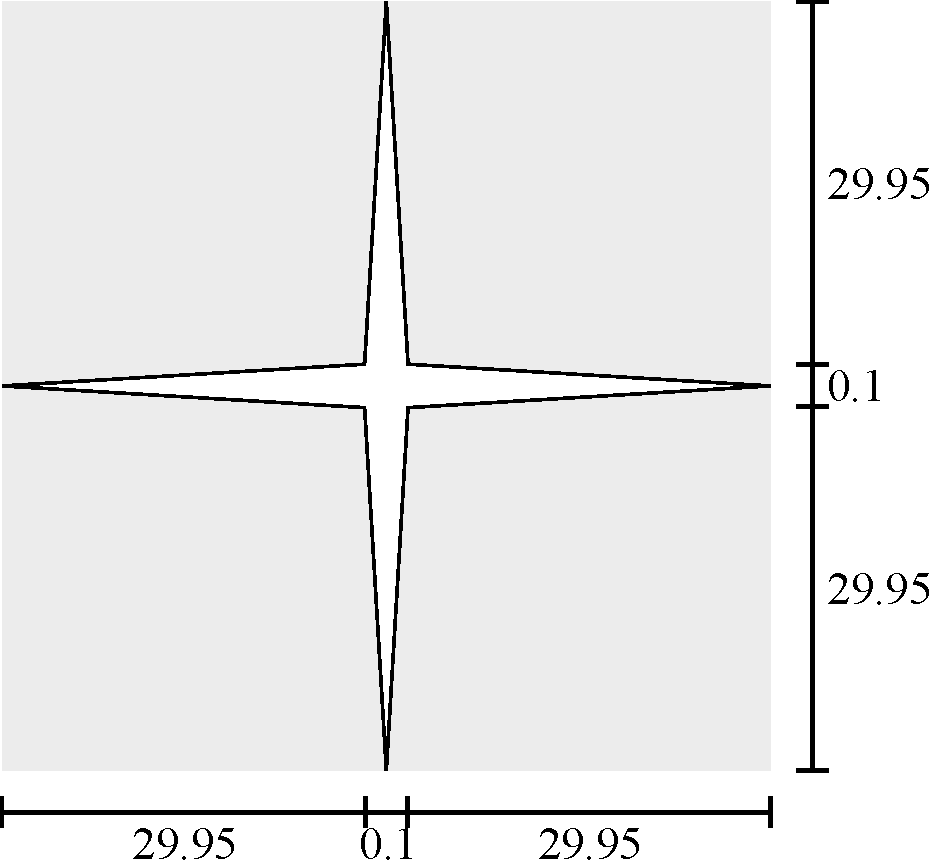
\includegraphics[width=\textwidth]{slit}
        \caption{}
        \label{fig:slit}
    \end{subfigure}
    \caption{Sketch of \text{(a)} blast exposed plates with four different slit defect geometries, and \text{(b)} the dimensions of the slits \text{(not drawn to scale)}. Measurements are in mm.}
\end{figure}

\begin{figure}
    \centering
    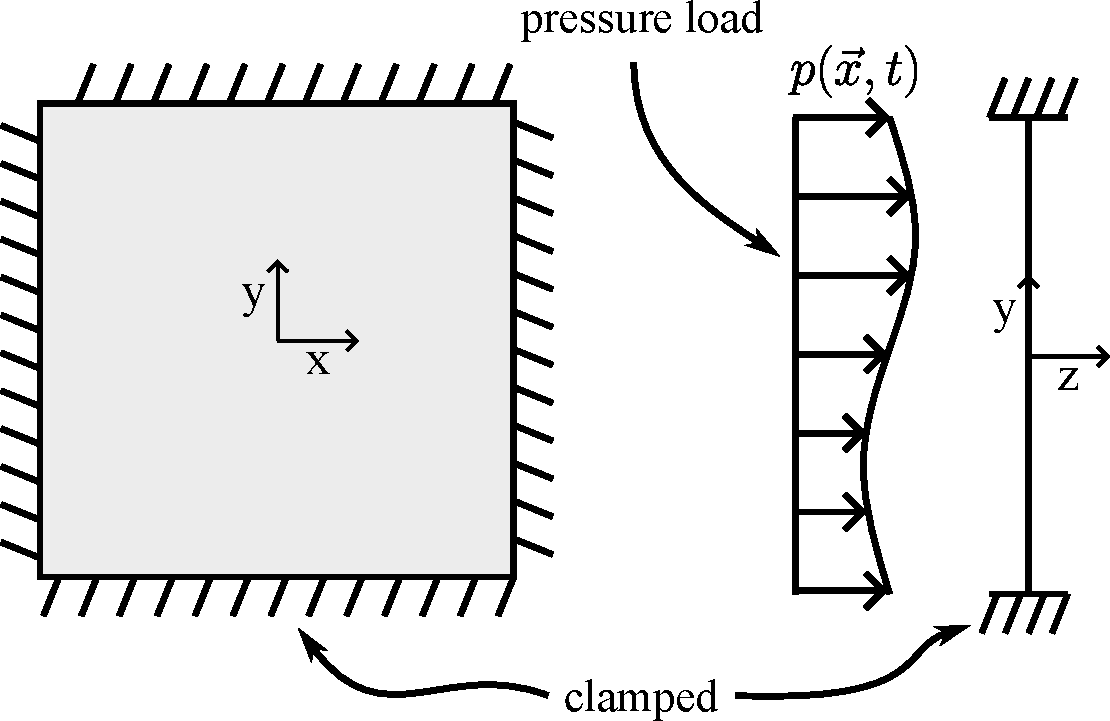
\includegraphics[width=.5\textwidth]{BC}
    \caption{Boundary and loading conditions. $p$ denotes pressure applied to one side, $\vec{x}$ denotes the position vector and $t$ is time}
    \label{fig:bc}
\end{figure}

\begin{figure}
    \centering
    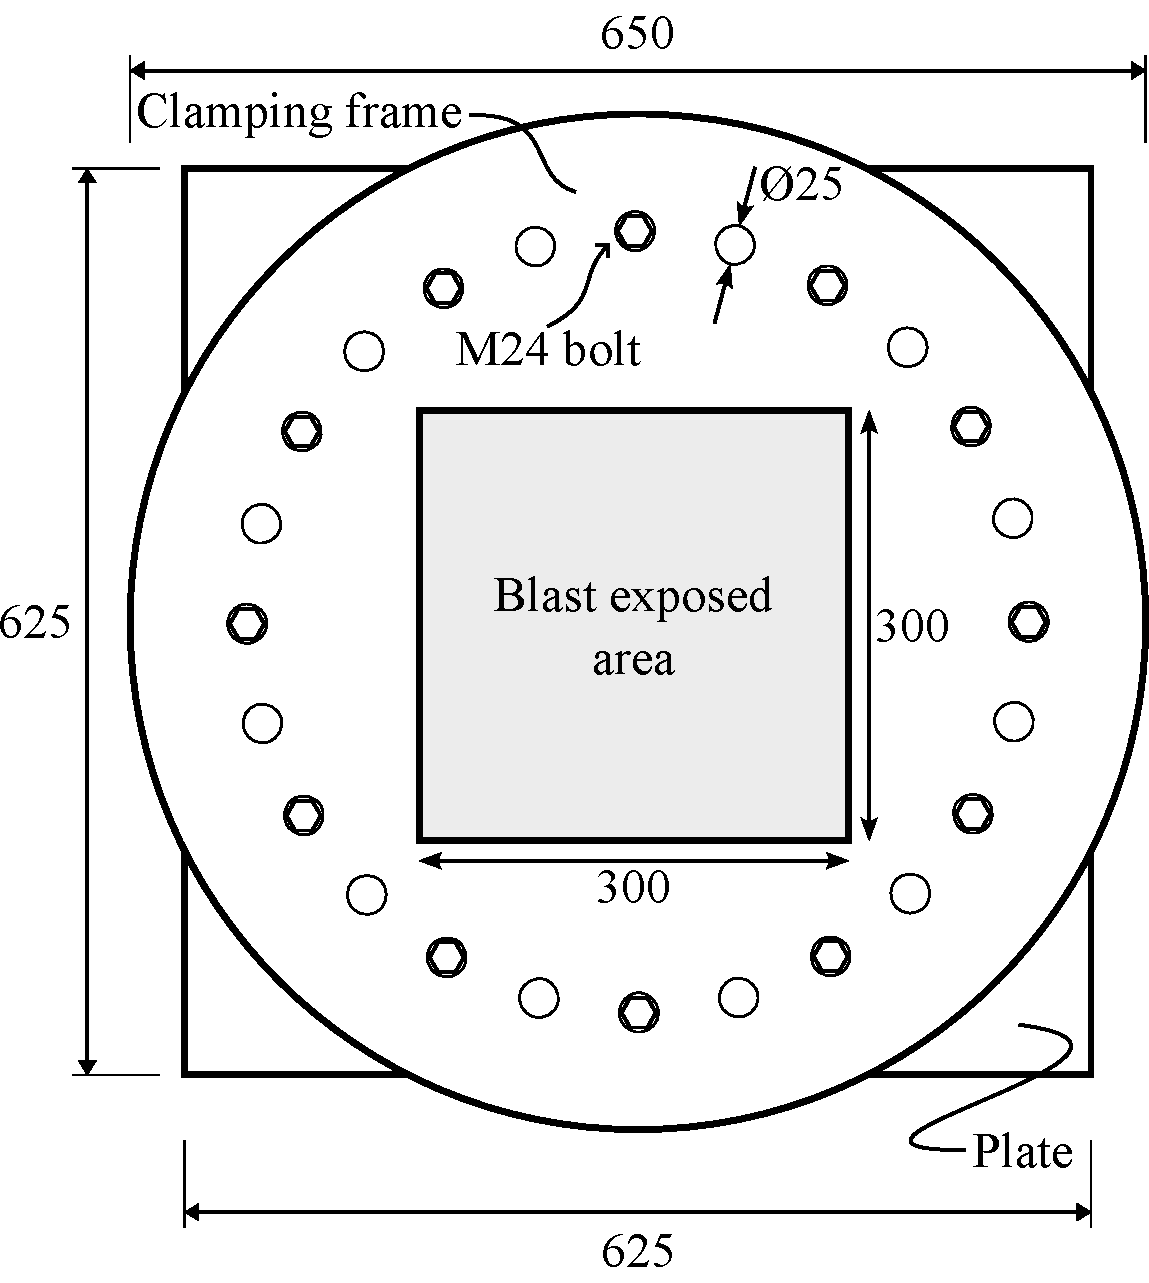
\includegraphics[width=.5\textwidth]{clamping_frame}
    \caption{Clamping frame}
    \label{fig:clamping}
\end{figure}